\chapter{Implementation}
\label{chap:implementation}

\section{Introduction}

This chapter describes the concrete realization of the AURA-MAS design as an open, tested Python codebase with 4{,}376 tracked Python lines (5{,}188 when uncommitted working-tree files are included). The evaluated configuration is the tracked code; the larger count is reported only to make the repository state explicit. We present the technology stack, the repository organization, the key algorithms of each component, and the engineering decisions that keep the system runnable on commodity hardware without any model training.

\section{Technology Stack}

\begin{table}[H]
\centering
\caption{Technology stack of the AURA-MAS prototype.}
\label{tab:stack}
\small
\begin{tabular}{p{3.5cm}p{4.2cm}p{5.3cm}}
\toprule
\textbf{Concern} & \textbf{Technology} & \textbf{Rationale} \\
\midrule
Language & Python 3.11+ & Ecosystem coverage of all required libraries \\
Detection + tracking & Ultralytics YOLO11n + ByteTrack \cite{ultralytics2025yolov8, zhang2022bytetrack} & Real-time on CPU; tracking integrated \\
Semantic anomaly & OpenAI CLIP ViT-B/32 \cite{radford2021clip} & Zero-shot; no training required \\
Audio & YAMNet \cite{tensorflow_yamnet} / librosa DSP fallback & Pretrained 521-class SED; light fallback \\
Event bus & MQTT (Mosquitto, paho-mqtt) \cite{light2017mosquitto} & Low-latency pub/sub, QoS, wildcards \\
Durable store & Redis Streams & Replayable alert/audit log \\
Explanation & OpenAI-compatible chat API & Works with GPT-4o-mini, Qwen-VL, local Ollama \\
Dashboard & Streamlit and Next.js console & Operator-facing alert views for prototyping and wall-display use \\
Testing & pytest & Offline tests without models \\
Deployment & Docker Compose & One-command broker setup \\
\bottomrule
\end{tabular}
\end{table}

The bus is hidden behind a small interface, \texttt{publish} and \texttt{subscribe} with MQTT-style wildcards. \texttt{LocalBus} implements the same interface, so the system and the auction can run in one process without external services. Heavy dependencies also have fallbacks: the audio agent uses \gls{dsp} when TensorFlow is unavailable, the camera agent can run rules without CLIP, and the explanation agent uses a template without an \gls{llm} endpoint. These choices keep the demonstrator runnable on a machine without the full production stack.

\section{Repository Organization}

\begin{verbatim}
aura_mas/
  core/       bus.py      (transports, Detection/Event/Alert schemas,
                           AlertStore with Redis/JSONL backends)
              privacy.py  (anonymization: person blurring, fail-closed)
  agents/     base.py     camera_agent.py   audio_agent.py
              fusion_agent.py  coordinator_agent.py
              policy_agent.py  explanation_agent.py
  scenarios/  replay.py   (scenario runner + centralized baseline)
  eval/       metrics.py  (event-level F1, time-to-alert, FAR/h, overhead)
  dashboard/  app.py      (Streamlit operator console)
  scripts/    make_synthetic_clips.py  probe_zones.py  make_figures.py
  tests/      offline unit and integration tests (26 tests; model-free subset available)
frontend/     Next.js operator console
scenarios/*.json   docker-compose.yml   requirements.txt
\end{verbatim}

\section{Core Components}

\subsection{Message Bus and Schemas}

\texttt{core/bus.py} defines the three dataclass schemas (Detection, Event, Alert) with \gls{json} serialization, topic constants, and three interchangeable transports: \texttt{MqttBus} (paho-mqtt), \texttt{LocalBus} (thread-safe in-process pub/sub with \texttt{+}/\texttt{\#} wildcard matching), and an \texttt{AlertStore} that appends alerts and audit records to Redis Streams when available, mirroring to JSONL files otherwise. Topic layout: \texttt{site/\{sensor\}/detections}, \texttt{site/events}, \texttt{site/coord/\{tasks,bids,awards,verifications\}}, \texttt{site/alerts}.

\subsection{Privacy Module}

\texttt{core/privacy.py} exposes a single choke point, \texttt{anonymize\_and\_save(frame, boxes)}, through which \emph{all} visual evidence must pass: person regions (YOLO boxes passed by the camera agent, or HOG fallback) receive strong Gaussian blurring of the head region plus lighter full-box blurring. If no person localization is available, the module \emph{fails closed} by blurring the entire frame. Raw frames are never written to disk.

\section{Agent Implementations}

\subsection{CameraAgent}

The camera loop reads frames, strides to the target inference rate, and calls \texttt{model.track(persist=True, tracker="bytetrack.yaml")}, yielding boxes with stable track identifiers in one call. The \texttt{ZoneRuleEngine} maintains dwell-time dictionaries keyed by (track, zone) and static-object records keyed by track, firing each rule at most once per key. The optional \texttt{ClipAnomalyScorer} encodes three ``normal'' and five ``anomalous'' text prompts once at startup; per sampled frame, the anomaly score is the softmax mass on anomalous prompts. It is retained as an experimental component, not a validated detector: its calibration AUC is 0.308 (Chapter~\ref{chap:evaluation}). For coordination, the agent subscribes to task announcements, computes its bid utility, and on award performs verification by re-running detection at \texttt{imgsz=960, conf=0.25} on its most recent frame, reporting the maximum person confidence found.

\subsection{FusionAgent and CoordinatorAgent}

The FusionAgent is callback-driven (one handler per incoming event) with a 1~Hz maintenance tick that flushes hypotheses whose window has closed; confidence follows Equation~\ref{eq:noisyor} exactly. The CoordinatorAgent implements the auction as: publish task, sleep the bidding window, select the maximal bid, publish award, and block (with timeout) on the verification topic---approximately 120 lines including the round-robin baseline and message accounting used by the evaluation.

\subsection{PolicyAgent}

The policy decision is a pure function of (severity map, thresholds, cooldown state, verification adjustment), executing in well under a millisecond; the measured decision latency in our runs averages 0.3~ms excluding verification rounds. Every code path terminates in an audit record.

\subsection{ExplanationAgent}

The explanation pipeline is implemented as four explicit methods (\texttt{collect}, \texttt{describe}, \texttt{draft}, \texttt{guardrail}) over a typed state object. The draft call requests \texttt{response\_format=json\_object} from the model; the guardrail validates schema completeness, then extracts all \texttt{ev\_*} identifiers from both the citation list and the free text via regular expression and checks set inclusion against the hypothesis's actual event identifiers. The unit test suite includes a hallucination probe verifying that a draft citing a fabricated identifier is rejected and the template fallback engages.

\section{Scenario Replay and Baselines}

\texttt{scenarios/replay.py} instantiates the full system from a \gls{json} manifest declaring sensors, zone polygons, and ground-truth events, then runs one of four modes: \texttt{mas-auction}, \texttt{mas-rules} (round-robin), \texttt{mas-nocoord} (coordination disabled), or \texttt{centralized}. The centralized baseline processes sensor sources \emph{sequentially in a single process}. The modes do not isolate architecture perfectly: \texttt{replay.py} paces MAS modes but not the centralized mode, while fusion windows and cooldowns are measured in wall-clock time. Time-to-alert comparisons must therefore be interpreted as confounded rather than as a pure concurrency measurement. Every run serializes alerts, ground truth, and per-agent metrics to a result \gls{json}.

\section{Evaluation Tooling and Dashboard}

\texttt{eval/metrics.py} matches alerts to ground-truth events by incident family and time tolerance ($\pm 5$~s), computing event-level precision/recall/F1, mean time-to-alert, false alerts per hour, and coordination overhead, and emits a summary CSV. The Streamlit console renders the alert feed with severity filtering, incident detail with the agentic report and anonymized evidence gallery, and acknowledge/dismiss buttons that write operator audit records. A separate Next.js console in \texttt{frontend/} provides an incident rail and wall-oriented view. Zone geometry and scenario-specific thresholds live in \texttt{scenarios/*.json}; the previously documented top-level \texttt{configs/} directory does not exist.

\begin{figure}[H]
\centering
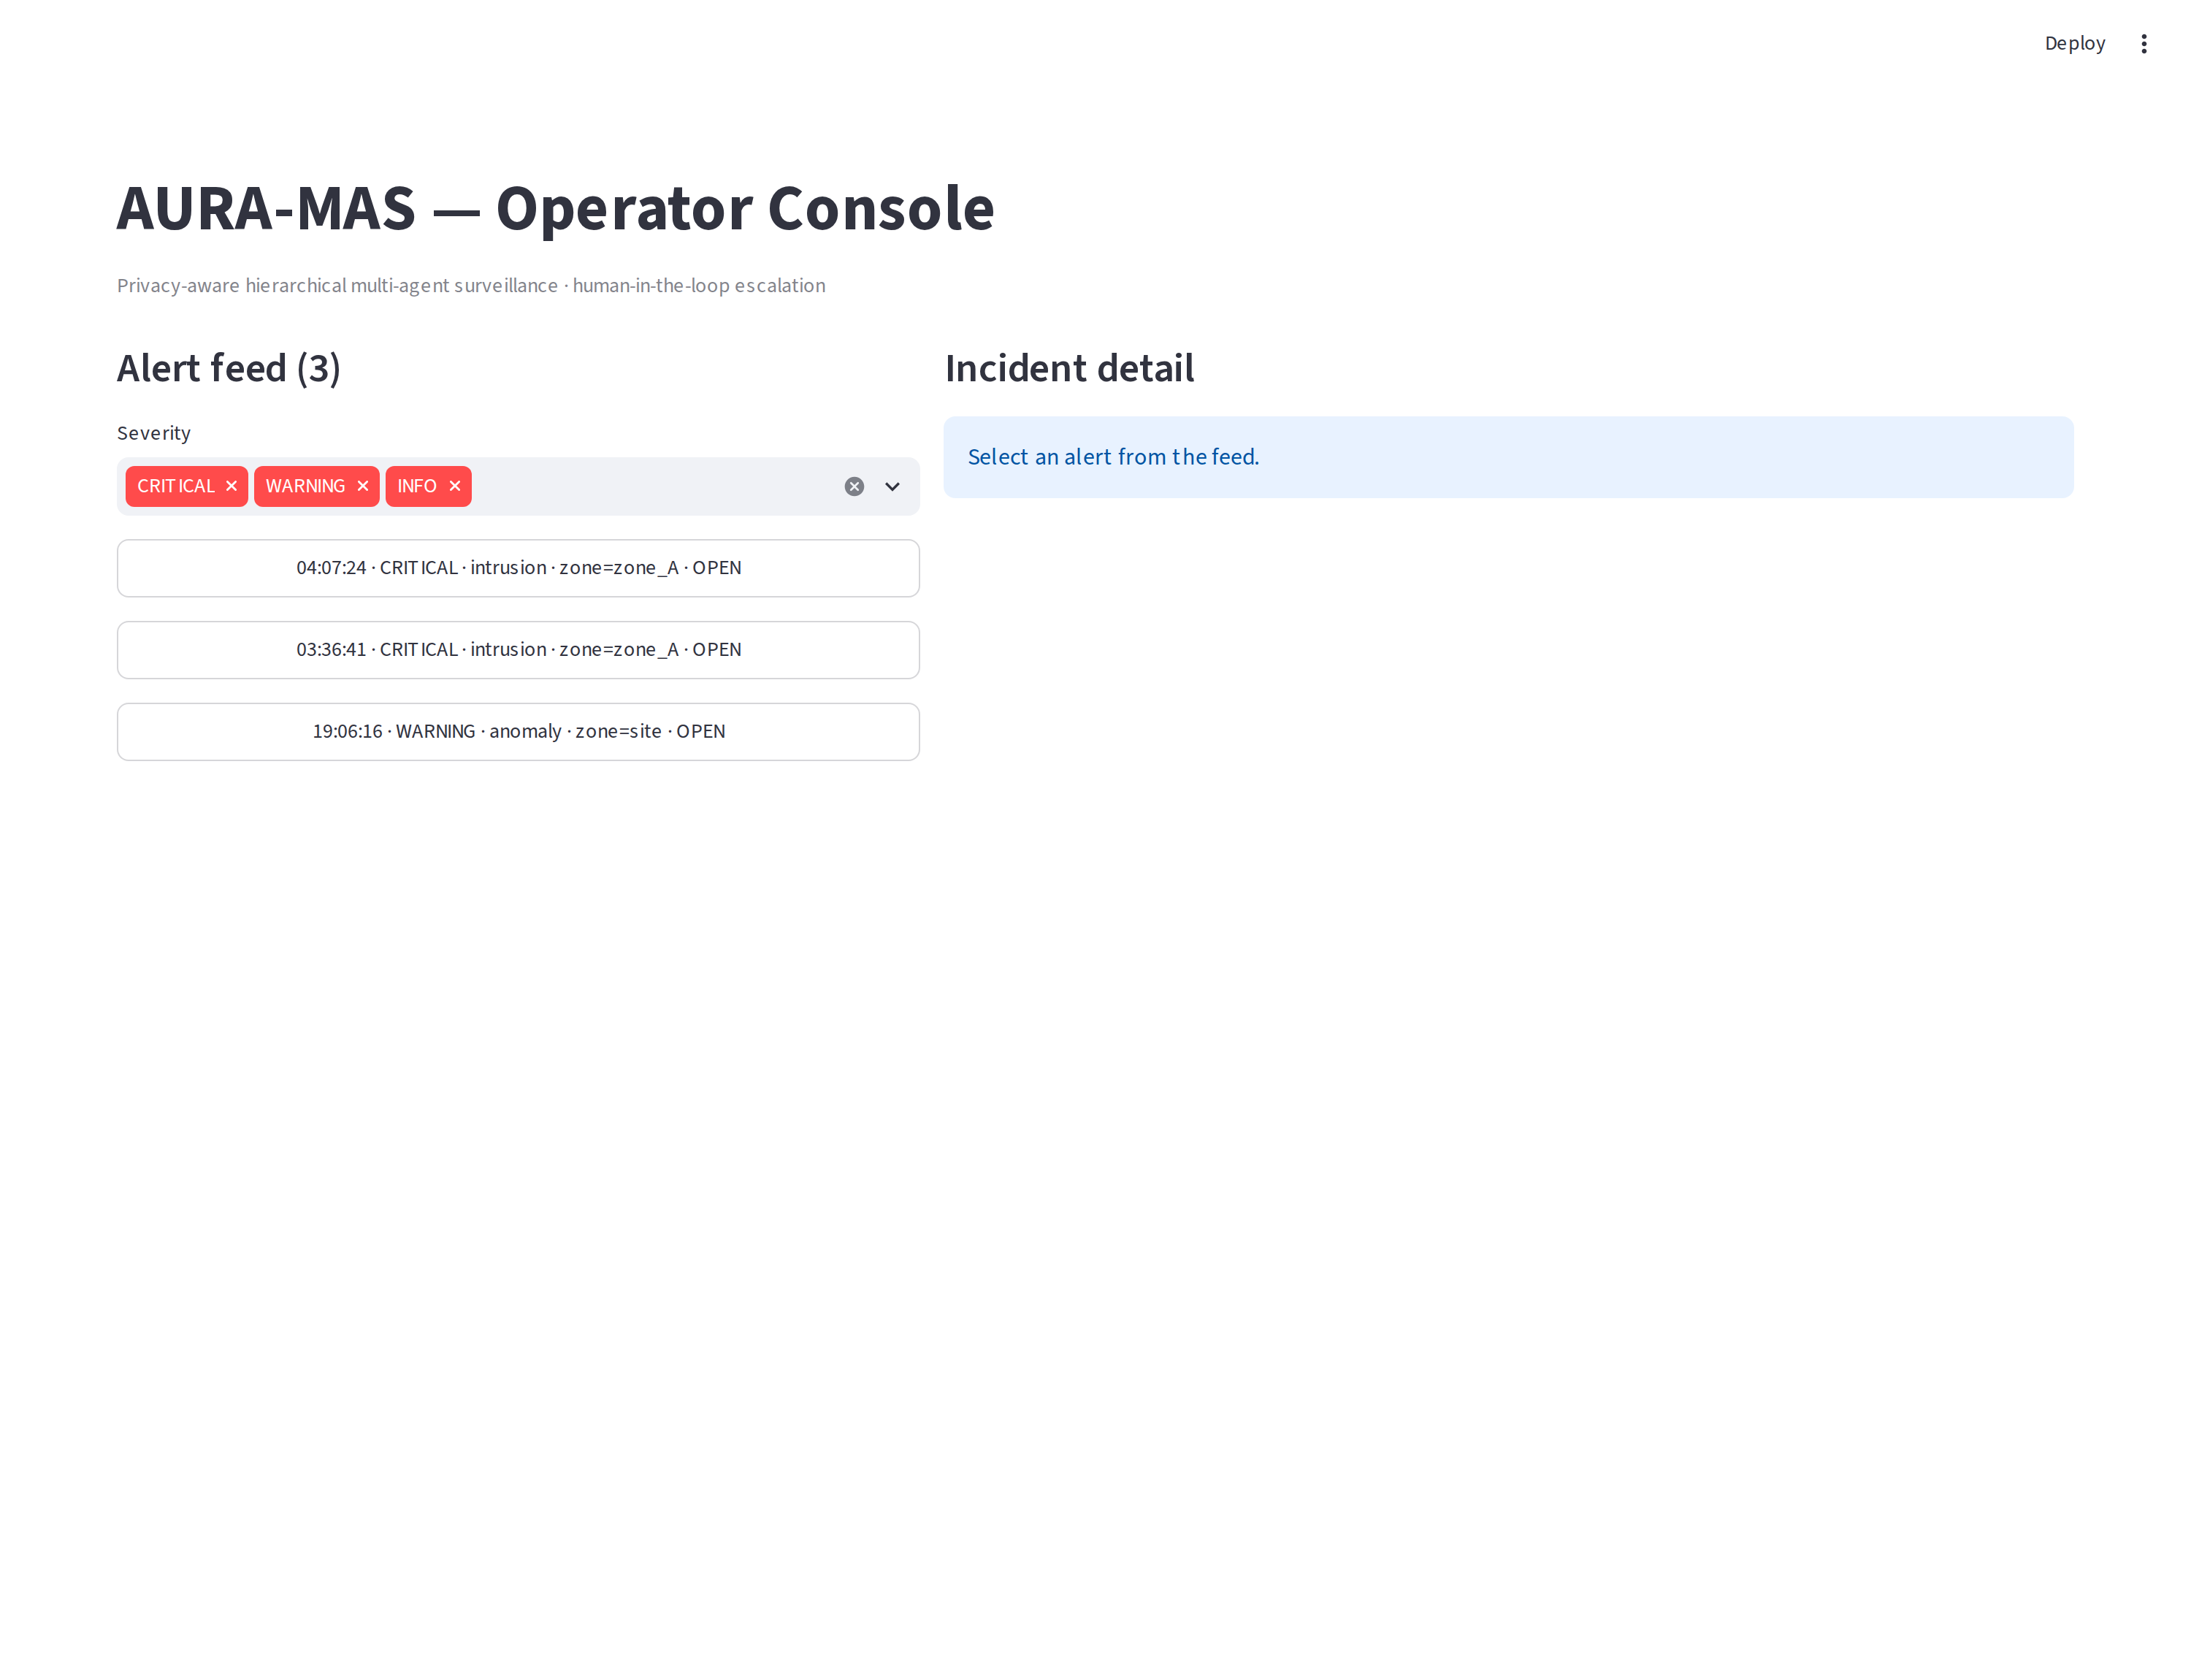
\includegraphics[width=0.82\textwidth]{Assets/shot_streamlit_console.png}
\caption{Live Streamlit operator-console capture reading local alert JSONL files. The view shows three open alerts: two CRITICAL intrusion alerts in \texttt{zone\_A} and one WARNING anomaly alert. This is a live interface capture, not a 373-run MQTT/Redis measurement.}
\label{fig:streamlit-console}
\end{figure}

\begin{figure}[H]
\centering
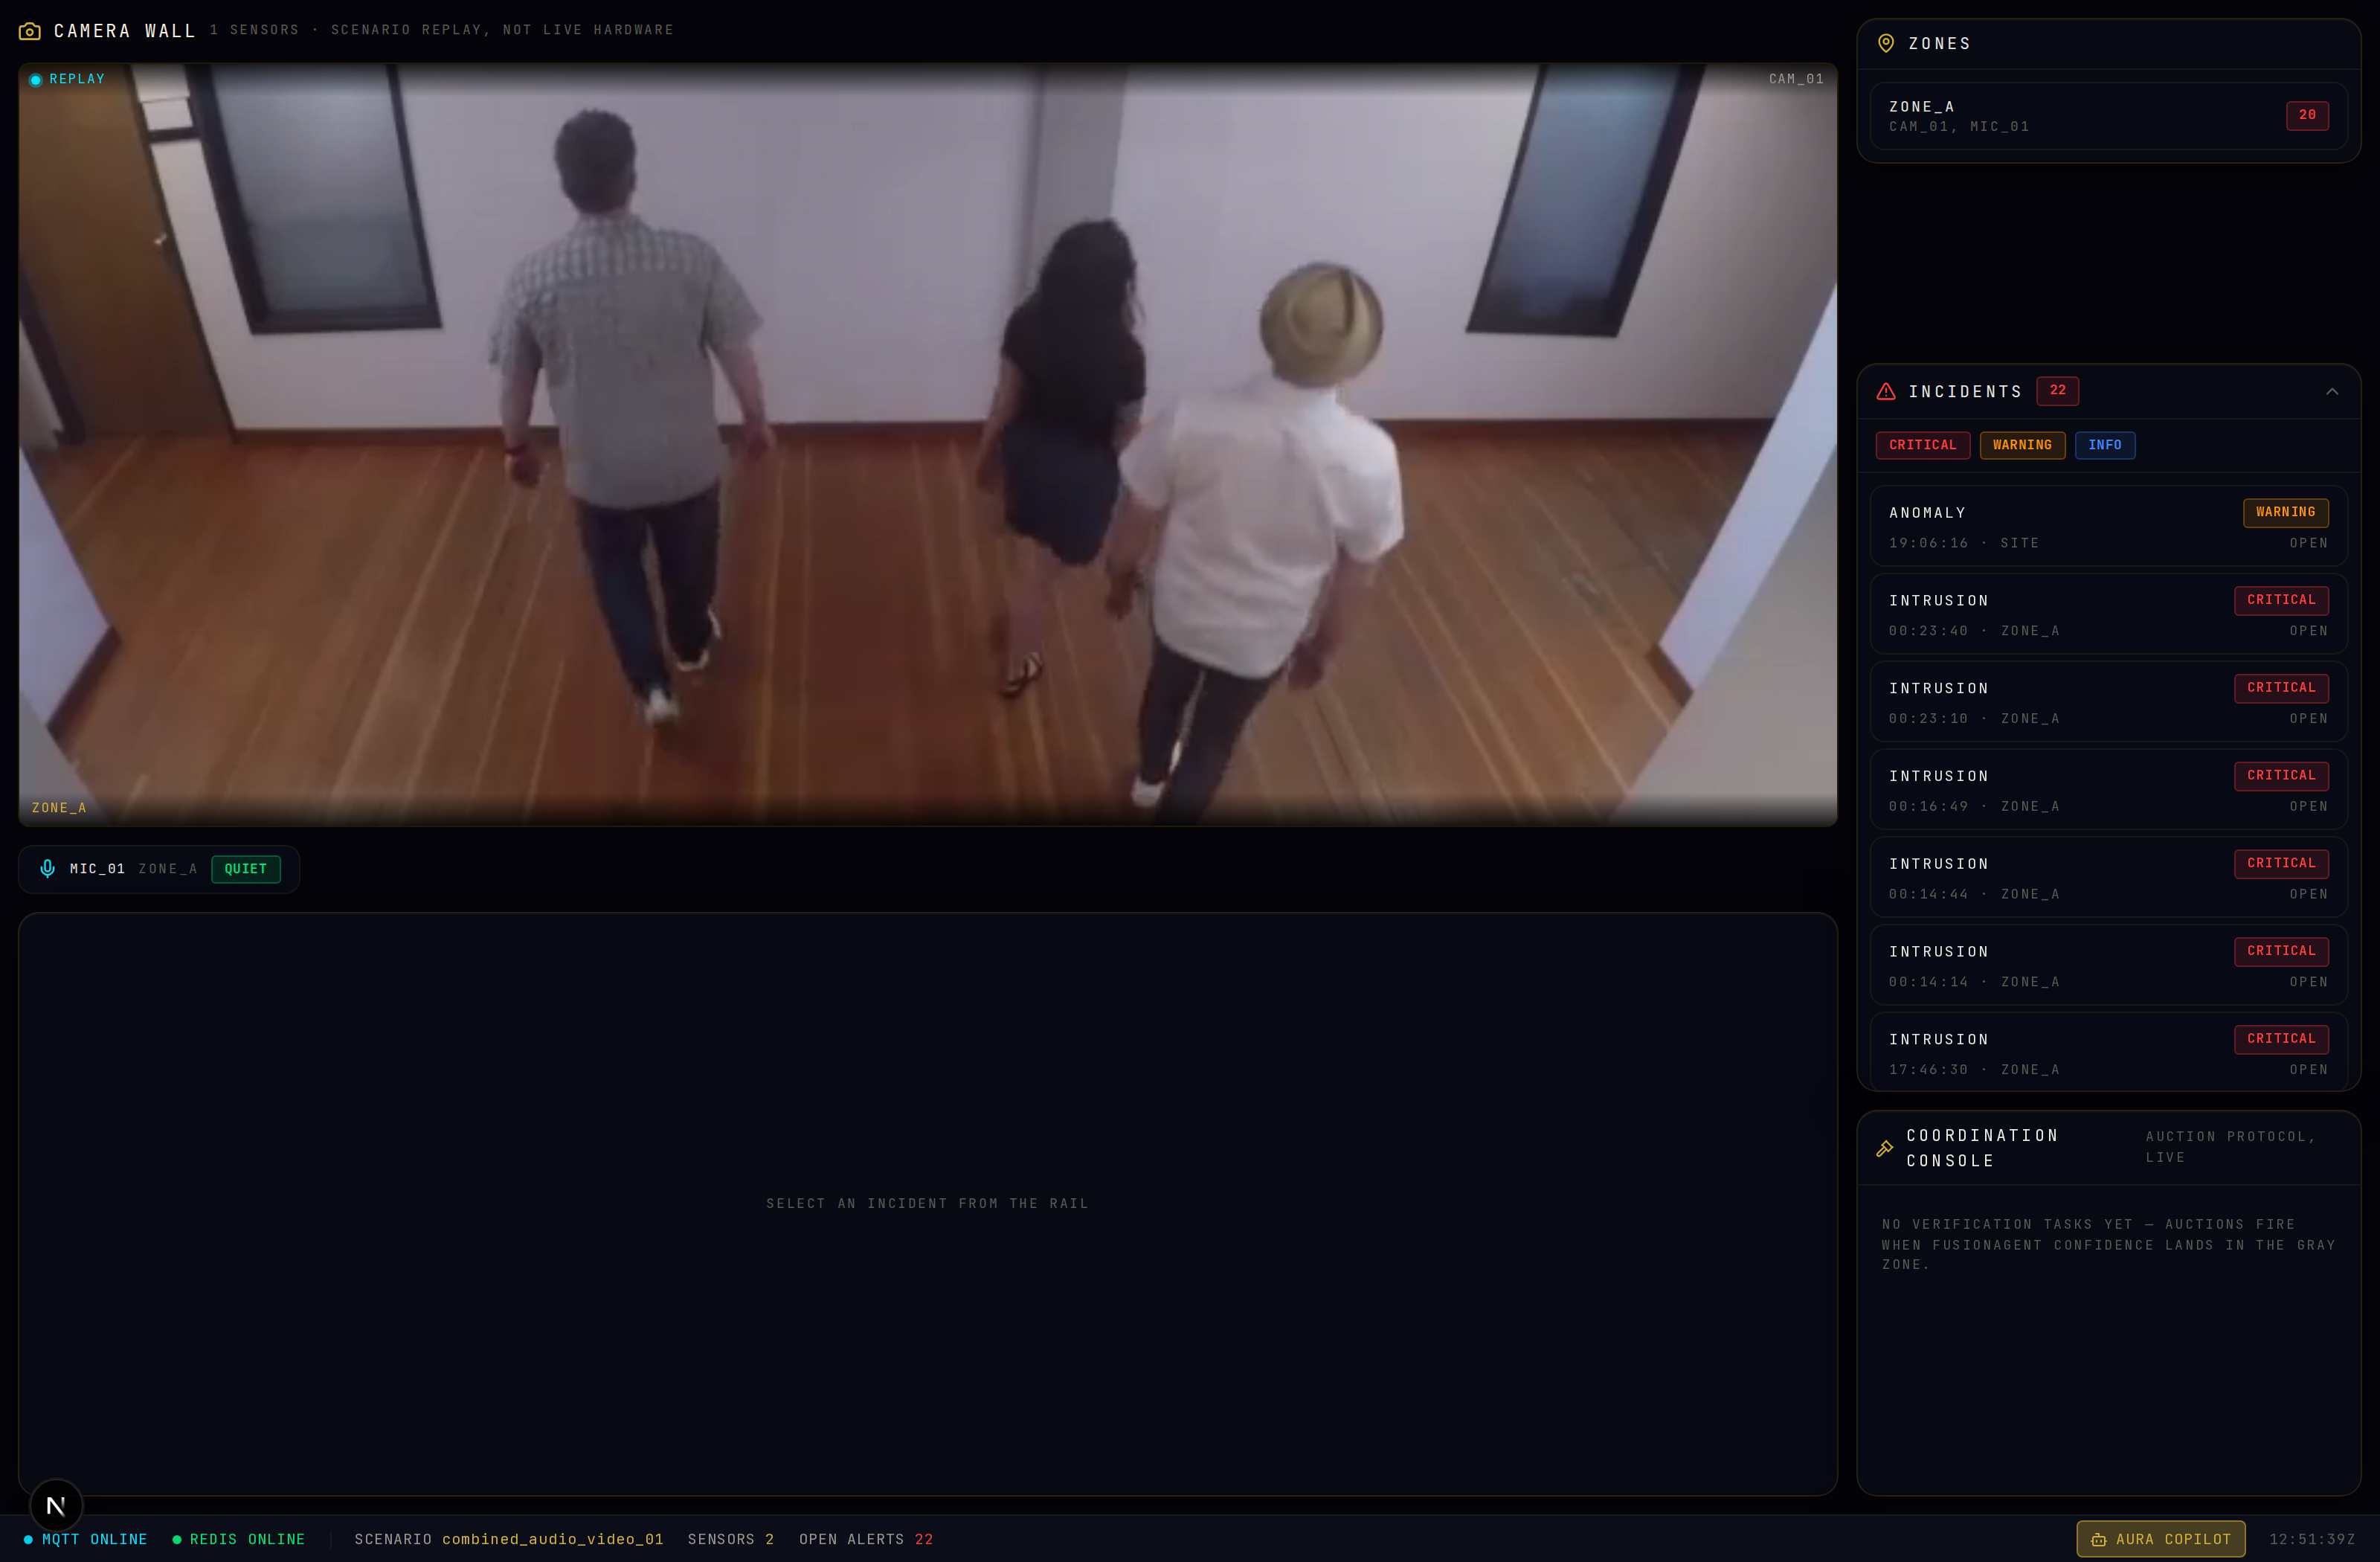
\includegraphics[width=0.92\textwidth]{Assets/shot_frontend_console.png}
\caption{Live Next.js operator-console capture for the \texttt{combined\_audio\_video\_01} replay. The status indicators describe the running local environment and must not be read as evidence that MQTT or Redis was exercised in the campaign, which used \texttt{LocalBus}.}
\label{fig:nextjs-console}
\end{figure}

\section{Testing}

The repository contains 26 offline tests. The model-free subset validates wildcard bus routing, monotone noisy-OR behaviour, auction best-bidder selection, policy thresholds and cooldown suppression, metric computation, and the guardrail hallucination probe. This supports test-driven iteration on coordination logic independently of perception, but it does not substitute for campaign evidence about performance.

\section{Conclusion}

The implementation provides the components described in Chapter~\ref{chap:design}, together with fallbacks, single-process tests, and serialized run artifacts. The next chapter evaluates those artifacts.
